%!TEX root = ../quantum.tex
\subsubsection{Нахождения волновой функции по данным одного из представлений}

$$\Psi(x)=\exp \qty{-\frac{(x-x')^2}{4b^2}+iUx} $$
В этом билете функция нормироваться не будет, так как автору стало лень, а на самом деле её и не просят. К тому же, на полу ширину нормировка не влияет.

$$\Psi(p)=\frac{1}{\sqrt{2\pi\hbar} } \infint \Psi(x) \exp{-\frac{ipx}{\hbar}}\dd{x} $$
Иначе говоря, $\Psi(p)=F[\Psi(x)]$.

По свойствам преобразования Фурье:  
\begin{enumerate}
	\item $\Psi_1(p-U\hbar)= F[\Psi_1(x)e^{iUx}]$ $\Psi_1(x)=\exp \qty{-\frac{(x-x')^2}{4b^2}}$
	\item $\Psi_2(p)\exp{-\frac{ipx'}{\hbar}}=F[\Psi_2(x-x')]$, где 
	$\Psi_2(x)=\exp \qty{-\frac{(x)^2}{4b^2}}$
\end{enumerate}

Найдем преобразование Фурье $\Psi_2(x)$ по определению.

\begin{gather*}
\Psi_2(p)=\frac{1}{\sqrt{2\pi\hbar}}\infint \exp{-\frac{x^2}{4b^2}+\frac{-ipx}{\hbar}}=\\
\frac{1}{\sqrt{2\pi\hbar}}\infint \exp{-\qty(\frac{x}{2b}+\frac{ipb}{\hbar})^2+
\qty(\frac{ipb}{\hbar})^2}\dd{x}= \\
\frac{1}{\sqrt{2\pi\hbar}}\exp{-\frac{p^2b^2}{\hbar^2}} 
\infint \exp{-\qty(\frac{x}{2b}+\frac{ipb}{\hbar})^2} \dd{x}=\\
\frac{2b}{\sqrt{2\pi\hbar}}\exp{-\frac{p^2b^2}{\hbar^2}} 
\infint \exp{-y^2}\dd{y}=\frac{2b\sqrt\pi}{\sqrt{2\pi b}}\exp{-\frac{p^2b^2}{\hbar^2}}=\\ 
\sqrt{\frac{2}{\hbar}}b\exp{-\frac{p^2b^2}{\hbar^2}}
\end{gather*}

Получим, что $\Psi_2(p)=\sqrt{\frac{2}{\hbar}}b\exp{-\frac{p^2b^2}{\hbar^2}}$.

$$\Psi_2(p)=F[\exp{-\frac{x^2}{4b^2}}]$$

Согласно свойству (2):
$$\sqrt{\frac{2}{\hbar}}b\exp{-\frac{p^2b^2}{\hbar^2}}\exp{-\frac{px'}{\hbar}}=
F[\Psi_2(x-x')]=F\qty[ \exp{-\frac{(x-x')^2}{4b^2}} ] = F[\Psi_1(x)]$$
Согласно свойству (1):
\begin{gather*}
\sqrt{\frac{2}{\hbar}}b\exp{-\frac{(p-U\hbar)^2b^2}{\hbar^2}}\exp{-\frac{i(p-U\hbar)x'}{\hbar}}=\\
 F\qty[\exp{-\frac{(x-x')^2}{4b^2}}+iUx]=F[\Psi(x)]
\end{gather*}
Что и требовалось найти.

\begin{equation}
	\Psi(p)=\sqrt{\frac{2}{\hbar}}b\exp{-\frac{(p-U\hbar)^2b^2}{\hbar^2}-\frac{i(p-U\hbar)x'}{\hbar} }
\end{equation}

Теперь найдем $\Delta p$. Она в $\Psi(p)$ такая же, как в $\Psi_2(p)$. Ищем полуширину на уровне $\frac{1}{e}$. Тогда
$$\Delta p=\frac{2\hbar}{b}$$
Найдем $\Delta x$на уровне $\frac1e$, при этом отбрасывая фазу.

\begin{gather*}
	-\frac{(x-x')^2}{4b^2}=-1 \\
	x_1=2b+x'\\
	x_2=x'-2b\\
	\Delta x= x_2-x_1=4b
\end{gather*}

$$\Delta x\cdot \Delta p=\frac{4b\cdot2\hbar}{b}=8\hbar  $$

\subsubsection{ {На примере конкретного пакета продемонстрируйте соотношение неопределенности. Операторы как матрицы. Непрерывные и дискретные индексы.} }

Зададим $C(p)$ следующим образом:
\begin{equation}
	C(p)=
	\begin{cases}
		C_0, & p \in (p_0- \Delta p, p_0+ \Delta p) \\
		0,   & p \in (-\infty, p_0- \Delta p)\cup(p_0+ \Delta p,\infty) \\
	\end{cases}
\end{equation}
И пусть $ \Delta p \ll p_0 $ (неопределенность импульса мала). Тогда в окрестности $p_0 $ справедливо
$$E(p)\approx  E_0+(p-p_0) \qty(\dv{E}{p})\eval_{p_0}.$$

Запишем функцию $\Psi$, отвечающую такой $C(p)$:
\begin{gather*}
	\Psi(x,t)=C_0\int\limits_{p_0+ \Delta p}^{p_0 - \Delta p}
	\frac{1}{\sqrt{2\pi\hbar}}\exp{i\frac{px-Et}{\hbar}}\dd{p}=
	\\
	\frac{C_0}{\sqrt{2\pi\hbar}} \int\limits_{p_0+ \Delta p}^{p_0 - \Delta p}
	\exp{i\frac{px-E_0t-(p-p_0)\dv{E}{p}\eval_{p_0}}{\hbar}} \dd{p} =\\
	\begin{pmatrix}
		\xi=\frac{p-p_0}{\hbar} \\
		\dd{p}=\hbar \dd{\xi}
	\end{pmatrix}=
	\frac{C_0\hbar}{\sqrt{2\pi\hbar}}\exp{i\frac{p_0x-E_0t}{\hbar}}
	\int\limits_{- \Delta p/\hbar }^{+\Delta p/\hbar}
	\exp{i\xi(x-\dv{E}{p}\eval_{p_0}t)}\dd{\xi}=\\
	\frac{C_0\hbar}{\sqrt{2	\pi \hbar}}\exp{i\frac{p_0x-E_0t}{\hbar}}f\qty(x-\dv{E}{p}t\eval_{p_0}),
\end{gather*}
где
$$f(\tilde x)= \int\limits_{- \Delta p/\hbar}^{+\Delta p/\hbar} e^{i\xi\tilde x}\dd{x}
=\frac{1}{i\tilde x}\eval^{\Delta p/\hbar}_{-\Delta p/\hbar}=\frac{2\sin(\frac{\Delta p \tilde x}{\hbar})}{\tilde x}$$
\begin{figure}[H]
\centering
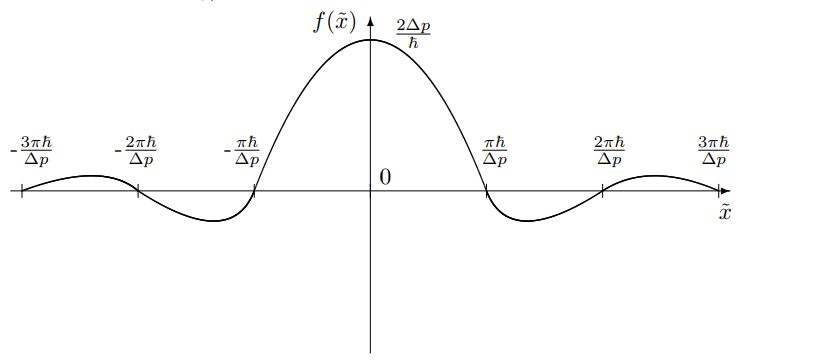
\includegraphics[width=0.7\linewidth]{fig/fig131}
\caption{}
\vspace{-17pt}
\end{figure}
Из графика сможем найти соотношение неопределенности
$$\Delta p \Delta x= 2\pi $$

\subsubsection{\textcolor{red} {Представления операторов умножения и дифференцирования как матриц.} }